\section{Lösungsansatz}
Bei der Berechnung der Entropie ist der zeitaufwendigste Teil im Code die Berechnung des Logarithmus.
% Daher haben wir zunächst beschlossen, die Anzahl der Logarithmusoperationen auf ein Minimum zu reduzieren, indem wir die Entropiefunktion (1) in eine riesige Logarithmusform bringen:
% \begin{equation*}
%         \text {Sei } X = \{x_{1},x_{2}, \cdots, x_{n}\}
% \end{equation*}
% \begin{equation*}
%     \mathrm {H} (X)= - \log_2 (\mathrm{P}(X=x_{1})^{\mathrm{P}(X=x_{1})} \cdot \mathrm{P}(X=x_{2})^{\mathrm{P}(X=x_{2})} \cdots \mathrm{P}(X=x_{n})^{\mathrm{P}(X=x_{n})})
% \end{equation*}
% Aber wir haben festgestellt, dass die Potenzfunktion mehr kostet als die Logarithmusfunktion, deshalb haben wir beschlossen, die Logarithmusfunktion für jede Wahrscheinlichkeit zu berechnen. \newline
Zur Berechnung der Logarithmusfunktion gibt es drei Hauptmethoden:
\begin{itemize}
    \item Approximation als Polynom
    \item Lookup Tabelle
    \item Approximation mit Hilfe von Lookup Tabelle (glibc Methode).
\end{itemize} 

Da wir mehrere Logarithmusfunktionen ausprobieren möchten, haben wir die Signatur der Entropiefunktion entsprechend erweitert. Man soll jetzt auch den Pointer der Logarithmusfunktion angeben.

Die Entropiefunktion an sich ist auch nicht direkt implementiert, wie von der Gleichung spezifiziert, sondern es nutzt die Kahan-Summe-Algorithmus.~\cite{kahan} Die Kahan-Summe hilft die Auslöschung bei einer Reihe von Additionen zu vermeiden.

\subsection{Approximation}
Der erste Ansatz an dieses Problem war, eine Polynomdarstellung der Logarithmusfunktion zu finden, die nicht aufwendig zu berechnen ist und auch für kleine Werte von $x$ schnell genug konvergiert.

Nach dem Testen einiger Möglichkeiten haben wir uns für zwei verschiedene Methoden zur Approximation der Logarithmusfunktion entschieden. Diese Methoden sollen leistungsfähig, präzise und vektorisierbar sein.

Da jede Gleitkommazahl die Form $x = 2^{k} \cdot z$ für ein $k \in \mathbb{Z}$ und $ z \in \mathbb{Q}$ hat, können wir zuerst den Exponenten extrahieren und dann Logarithmus für $z$ berechnen die zwischen $1$ und $2$ liegt.
\[\log_2{x} = k + \frac{\ln{z}}{\ln{2}}\]
Bei den folgenden Approximierungsmethoden haben wir immer berücksichtigt, wie anpassungsfähig diese Methoden an die SIMD-Version sind, was für den Performance-Gewinn eine große Rolle spielen wird.

\subsubsection{ARTANH Approximation}
Wir können $\ln(x)$ als eine  konvergente Summe von Potenzreihen schreiben, indem wir die Taylorreihe von $\artanh$ verwenden. Die Partialsumme der Potenzreihe konvergiert für kleine Werte von $x$ schneller als die normale Taylorreihe von $\ln(x)$.
\begin{equation}
    \ln(x) = 2 \cdot \artanh\left(\frac{x-1}{x+1}\right) = 2\left(\sum _{k=0}^{\infty}{\frac{1}{2k+1} \cdot \left(\frac{x-1}{x+1}\right)^{2k+1}}\right)
\end{equation}

\begin{equation}
   \text{Sei }  S_{n} = 2\left(\sum _{k=0}^{n}{\frac{1}{2k+1} \cdot \left(\frac{x-1}{x+1}\right)^{2k+1}}\right)
   \label{eq:artanh}
\end{equation}

Obwohl die Artanh-Approximation eine Division erfordert, ist der absolute Unterschied zwischen Logarithmusfunktion und Artanh-Approximation mit $S_{2}$ fast $0$, wenn die Zahl zwischen $1$ und $2$ liegt.

\subsubsection{Remez Algorithmus}
Der Remez-Algorithmus ist ein Minimax-Approximations-Algorithmus, das die maximale absolute Differenz zwischen dem Polynom und der gegebenen stetigen Funktion im Intervall $[a,b]$ minimiert ~\cite{remez}.

Um Polynome zur Approximation von $\ln(x)$ im Intervall $[1,2)$ zu erzeugen, haben wir ein Open-Source-Projekt namens „lolremez“~\cite{lolremez} verwendet.
Wir haben 2 verschiedene Polynome mit dem Grad $2$ und $4$ implementiert.

\begin{equation}
    \mathrm{P_{2}}(z) = -0.344845 \cdot z^{2}+ 2.024658 \cdot z -1.674873
    \label{eq:deg2}
\end{equation}

\begin{equation}
    \mathrm{P_{4}}(z) = -0.081616z^{4} + 0.645142z^{3} -2.120675z^{2} + 4.070091z -2.512854
    \label{eq:deg4}
\end{equation}

Das Polynom mit Grad $2$ liefert ungenauere Ergebnisse, gewinnt aber auch etwas an potenzieller Geschwindigkeit, da es $2$ Multiplikationen weniger hat.

\subsection{Lookup Tabelle }
Ein anderer Ansatz besteht darin, eine sogenannte Lookup Tabelle zu benutzen. Anstatt dass wir der in Mantisse gespeicherte Wert zu $log_2(x)$ annähern, speichern wir vorher diese Werte in einer Tabelle und geben sie zurück gemäß der Mantisse. Für das Erhalten der Genauigkeit von $100\%$ brauchen wir insgesamt $2^{23}$ Einträge in der Tabelle, welche aber nämlich 
\[2^{23} . 4 \text{ bytes } = 2^{15} \text{ Kb } = 32 \text{ Mb }\]

Unter Berücksichtigung das Experiment von der Universität Berkeley ~\cite{fast_log} haben wir uns entschieden, nur erste $16$ bits von der Mantisse für die Tabelle zu benutzen und die letzten $7$ bits zu ignorieren.

\begin{figure}[h]
    \centering
    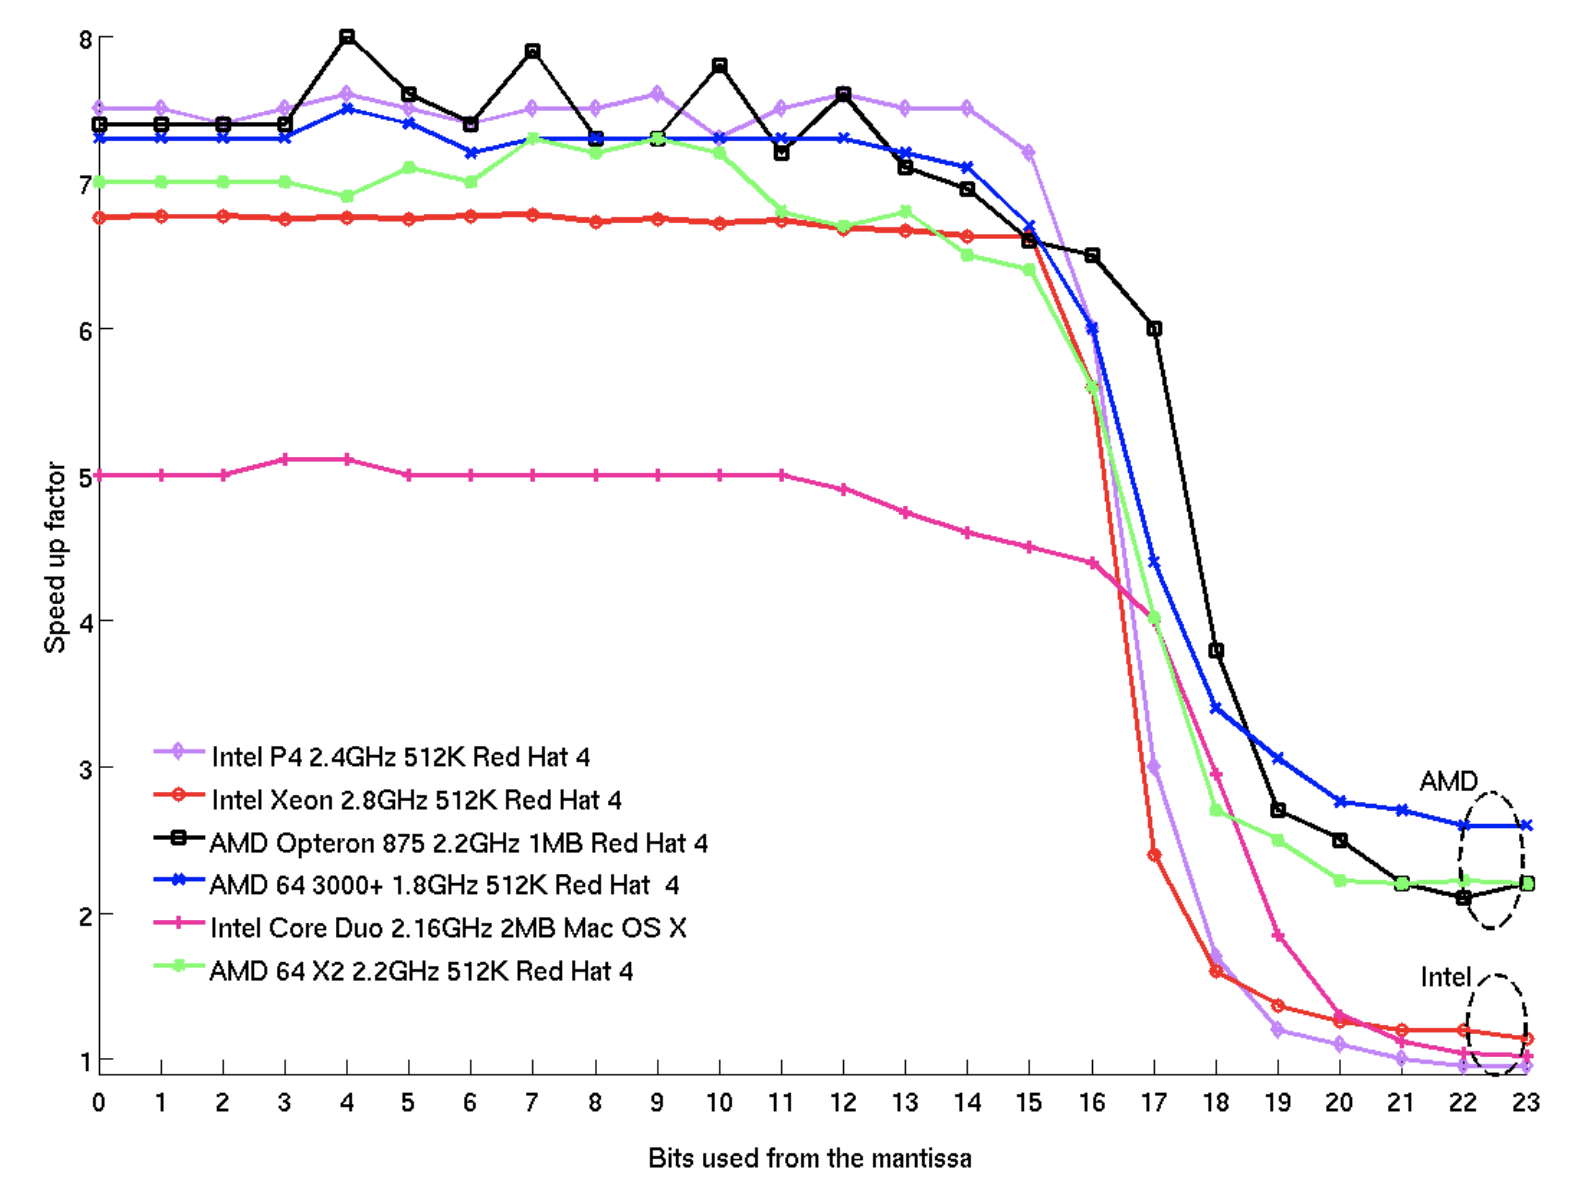
\includegraphics[scale=0.35]{lookup_berkeley.png}
    \caption{Performanz-Genauigkeit Trade-Off der logf mit Lookup Tabelle auf unterschiedliche Systeme}
    \label{graph:lookup_berkeley}
\end{figure}

Weil wir die Tabelle somit verkleinert haben, können wir die Cache effizienter benutzen um Performanz zu erhöhen, jedoch verlieren wir die Genauigkeit im Durchschnitt um $6.55 \cdot 10^{-6}$. Das ist einer der Trade-Offs, die wir während der Entwicklung begegnet und sie werden in folgender Abschnitte eingegangen.
 
\subsection{Glibc - log2f}
Die glibc Implementierung von $log2f$ nutzt eine Kombination von Approximation und Lookup Tabelle. Erst ist x in Mantisse $z$ und Exponent $k$ geteilt.

\[log_2(x) = log_2(2^k \cdot z) = k + log_2(z) \]

Mittels z ist ein Index berechnet, mit dem man in der Lookup-Tabelle eine Variable c ($\approx z$) und $log_2(c)$ findet.

\[log_2(x) = k + log_2(z/c) + log_2(c)\]

Jetzt muss man nur $log_2(\frac{z}{c})$ berechnen, das wird durch die Taylor-Reihe approximiert. Das liefert genaue Ergebnisse, weil $\frac{z}{c}$ sehr nähe zu $1$ ist, wo die Taylor-Reihe sehr schnell konvergiert. 

% Die glibc Implementierung von $log2f$ nutzt eine Kombinitaion von Approximation und Lookup Tabelle. Erst wird die Zahl $x$ in Form $2^k\cdot z$ gebracht, wo $k \in \mathbb{Z}$ und $\ln2 \leq z \leq 2\cdot\ln2$. Dann wird diese Interval in $16$ Subintervals geteilt. 

% Mittels $z$ kann man berechnen, in welcher Subinterval $z$ liegt. Der Mittelpunk dieser Subinterval ist $c$. Die Werte $\frac{1}{c}$ und $\log_2(c)$ in der Tabelle gespeichert. Außerdem wird die Taylor Series von Grad $4$ benutzt, um $f(x) = \log_2(x + 1)$ zu approximieren. Jetzt ist es zu berechnen: \[\log_2(x) = f(\frac{z}{c} - 1) + \log_2(c) + k\]

% Weil die Zahl $\frac{z}{c} - 1 \approx 0$, konvergiert Taylor Series sehr schnell und liefert $log2f$ ein sehr präzises Ergebnis.

\subsection{SIMD}
Für unsere Algorithmen sind Optimierungen durch SIMD deutlich möglich und sinnvoll. SIMD-Befehle nutzen XMM Registern, die $128$ Bits haben. Unsere Algorithmen arbeiten mit Fließkommazahlen, die $32$ Bits haben. Daher können wir mittels SIMD-Befehle $4$ Einträge gleichzeitig bearbeiten. Dadurch kann man ein theoretischen maximalen Speedup von $4$ erreichen.

% Um unnötige Überprüfungen in unsere SIMD-Implmentation zu vermeiden, erweitern wir das Array der Fließkommazahlen, sodass die Länge durch 4 trennbar ist. Die zusätzliche Zahlen sind alle $0$ und sie verändern nicht das Endergebnis. Außerdem allozieren wir das Array 16-Byte-Aligned, dann können wir Befehle, wie z.B. \emph{movaps}, nutzen, die effizienter sind als ihre unaligned Gegenstücke.

% Der SIMD Entropie Algorithmus funktioniert wie folgt:
% \begin{enumerate}
%     \item In einem XMM-Register, SUM, sind 4 Fließkommazahlen geladen, die gleich 0 sind.
%     \item In eine Schleife von 0 bis n-1 mit Schrittweite 4, sind 4 Einträge von das Array gelesen.
%     \item Der Logarithmus der Einträge ist berechnet und mit den Einträgen multipliziert.
%     \item Die Werte der Multiplikation sind dann auf dem Register SUM subtrahiert.
%     \item Nach der Schleife, sind die Einträge der Register SUM horizontal addiert und zurückgegeben.
% \end{enumerate}

Natürlich sind die Logarithmusfunktionen ebenfalls vektorisiert. Hier wird einer der größten Vorteile der Verwendung von Approximationen deutlich. Die Approximationsfunktionen verwenden nur eine Reihe von sehr einfachen Operationen, wie z.B. Addition, Multiplikation, Bitverschiebung und so weiter. Diese Operationen sind in SIMD mit wenig bis gar keinem Overhead replizierbar. Daher ist es möglich, sich dem maximalen Speedup anzunähern.

Im Gegensatz dazu ist die Vektorisierung von der Lookup-Version unsere Logarithmusfunktion deutlich ineffizienter. Den Index zu finden für jeden Eintrag, kann man noch gut vektorisieren. Mit 2 Befehle findet man das Index von alle 4 Einträge. Nachdem man die Indices hat, muss man jeden Eintrag der Lookup-Tabelle einzeln in das Register laden. Da diese Einträge in der Lookup-Tabelle höchstwahrscheinlich weit voneinander entfernt sind, fallen viele Cache-Misses an. 

\subsection{Umgang mit denormalen Zaheln}
Um die oben beschriebenen Methoden an die denormalen Zahlen anzupassen ist eine spezielle Behandlung benötigt. Unsere Methoden funktionieren für die Zahlen $x = 2^k \cdot z$ wo $1 \leq z < 2$. Bei den denormalizierten Zahlen liegt $z$ im Interval $[0,1)$, wo unsere Approximationen sehr ungenau sind. Deswegen müssen die denormalen Zahlen erst normaliziert werden. 

Dafür multiplizieren wir die Zahlen mit $2^{23}$, deren Exponent gleich $0$ ist. Unsere Zahl ist damit normaliziert, aber ist jetzt $2^{23}$ mal mehr als wir erwarten würden. \[log_2(x\cdot 2^{23}) = log_2(x) - log_2(2^{23}) = log_2(y) - 23\]
Aus diesem Grund subtrahieren wir $23$ von dem Exponent und führen wir die normalen Schritte für die Logarithmusfunktion.

% Für SIMD ist der Ansatz gleich, aber die Methode ändert sich denn ein Vergleich für einzelne Zahlen ist nicht mehr möglich. Wohingegen werden die normalen Zahlen mit $1.0$ und denormalen Zahlen mit $2^{23}$ multipliziert und von deren Exponent 23 subtrahiert. Die Bitmasken dafür sehen wie folgt aus:

% \[
% \begin{array}{ccc}
%      1.0f & : & 0\;01111111\;00000000000000000000000  \\
%     2^{23}f & : & 0\;10010110\;00000000000000000000000 \\
%     \text{xor Maske}: & : & 0\;11101001\;00000000000000000000000
% \end{array}
% \]

% Die Masken aus $pcmpeqd$ mit $0$ werden erst mit xor-Masken andet, dann wird das Ergebnis mit $1.0f$ xored. Die Resultat ist $1.0f$ für normalizierte Zahlen und $2^{23}$ für denormale Zahlen.
% Am Ende wird die zu logierende Zahlen mit diesem Ergebnis multipliziert.

% \subsection{Glibc (just draft for us)}
% \[x = 2^k . z\] where \[ln2 \leq z < 2ln2\]

% \[log1p(x) = \ln{x + 1}\]

% with

% \[log1p(\frac{z}{c} - 1) + log_2(c) = \ln{(\frac{z}{c})}+ log_2(c) = \ln{(z)}\]

% then

% \[log_2(x) = \frac{\ln{(\frac{z}{c})}+ log_2(c)}{\ln2} + k\]

% to approximate $\ln(x + 1)$ they use Taylor Series of 4th degree.

% So we need to figure out what is c, because $\frac{z}{c}$ is a number which is really close to 1